% This file was created by tikzplotlib v0.9.5.
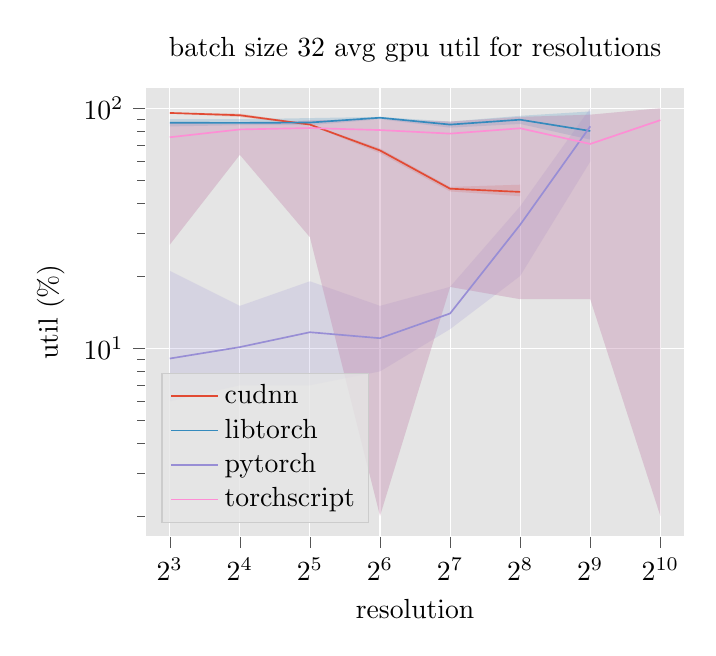
\begin{tikzpicture}

\definecolor{color0}{rgb}{0.886274509803922,0.290196078431373,0.2}
\definecolor{color1}{rgb}{0.203921568627451,0.541176470588235,0.741176470588235}
\definecolor{color2}{rgb}{0.596078431372549,0.556862745098039,0.835294117647059}
\definecolor{color3}{rgb}{0.984313725490196,0.756862745098039,0.368627450980392}
\definecolor{torchscript}{rgb}{0.996078431372549,0.556862745098039,0.835294117647059}

\begin{axis}[
axis background/.style={fill=white!89.8039215686275!black},
axis line style={white},
legend cell align={left},
legend style={fill opacity=0.8, draw opacity=1, text opacity=1, at={(0.03,0.03)}, anchor=south west, draw=white!80!black, fill=white!89.8039215686275!black},
log basis y={10},
tick align=outside,
tick pos=left,
title={batch size 32 avg gpu util for resolutions},
x grid style={white},
xlabel={resolution},
xmajorgrids,
xmin=2.65, xmax=10.35,
xtick style={color=white!33.3333333333333!black},
y grid style={white},
ylabel={util (\%)},
ymajorgrids,
ymin=1.64468031885378, ymax=121.604179065866,
ymode=log,
ytick style={color=white!33.3333333333333!black},
xticklabels={$2^3$, $2^4$, $2^5$, $2^6$, $2^7$, $2^8$, $2^9$, $2^{10}$},
xtick={3,...,10},
]
\path [fill=color0, fill opacity=0.2, very thin]
(axis cs:3,96)
--(axis cs:3,95)
--(axis cs:4,92)
--(axis cs:5,85)
--(axis cs:6,65)
--(axis cs:7,45)
--(axis cs:8,43)
--(axis cs:8,48)
--(axis cs:8,48)
--(axis cs:7,47)
--(axis cs:6,68)
--(axis cs:5,86)
--(axis cs:4,95)
--(axis cs:3,96)
--cycle;

\path [fill=color1, fill opacity=0.2, very thin]
(axis cs:3,90)
--(axis cs:3,84)
--(axis cs:4,85)
--(axis cs:5,85)
--(axis cs:6,90)
--(axis cs:7,83)
--(axis cs:8,86)
--(axis cs:9,74)
--(axis cs:9,97)
--(axis cs:9,97)
--(axis cs:8,93)
--(axis cs:7,88)
--(axis cs:6,92)
--(axis cs:5,91)
--(axis cs:4,90)
--(axis cs:3,90)
--cycle;

\path [fill=color2, fill opacity=0.2, very thin]
(axis cs:3,21)
--(axis cs:3,6)
--(axis cs:4,7)
--(axis cs:5,7)
--(axis cs:6,8)
--(axis cs:7,12)
--(axis cs:8,20)
--(axis cs:9,60)
--(axis cs:9,100)
--(axis cs:9,100)
--(axis cs:8,39)
--(axis cs:7,18)
--(axis cs:6,15)
--(axis cs:5,19)
--(axis cs:4,15)
--(axis cs:3,21)
--cycle;

\path [fill=white!46.6666666666667!black, fill opacity=0.2, very thin]
(axis cs:3,87)
--(axis cs:3,27)
--(axis cs:4,64)
--(axis cs:5,29)
--(axis cs:6,2)
--(axis cs:7,18)
--(axis cs:8,16)
--(axis cs:9,16)
--(axis cs:10,2)
--(axis cs:10,100)
--(axis cs:10,100)
--(axis cs:9,94)
--(axis cs:8,92)
--(axis cs:7,88)
--(axis cs:6,90)
--(axis cs:5,89)
--(axis cs:4,86)
--(axis cs:3,87)
--cycle;

\path [fill=torchscript, fill opacity=0.2, very thin]
(axis cs:3,87)
--(axis cs:3,27)
--(axis cs:4,64)
--(axis cs:5,29)
--(axis cs:6,2)
--(axis cs:7,18)
--(axis cs:8,16)
--(axis cs:9,16)
--(axis cs:10,2)
--(axis cs:10,100)
--(axis cs:10,100)
--(axis cs:9,94)
--(axis cs:8,92)
--(axis cs:7,88)
--(axis cs:6,90)
--(axis cs:5,89)
--(axis cs:4,86)
--(axis cs:3,87)
--cycle;

\addplot [semithick, color0]
table {%
3 95.5999984741211
4 93.5
5 85.4999923706055
6 66.6999893188477
7 46.2000007629395
8 44.7999992370605
};
\addlegendentry{cudnn}
\addplot [semithick, color1]
table {%
3 87.0000076293945
4 86.9000015258789
5 87.1999969482422
6 91.3000030517578
7 85.4999923706055
8 89.6000137329102
9 80.3999938964844
};
\addlegendentry{libtorch}
\addplot [semithick, color2]
table {%
3 9.05000019073486
4 10.0999994277954
5 11.6499996185303
6 11
7 13.9499988555908
8 32.6999969482422
9 84.0500106811523
};
\addlegendentry{pytorch}
\addplot [semithick, torchscript]
table {%
3 75.7000045776367
4 81.5999908447266
5 82.6999969482422
6 81.1000061035156
7 78.4000015258789
8 82.5
9 71.0000076293945
10 89.1999969482422
};
\addlegendentry{torchscript}
\end{axis}

\end{tikzpicture}
